\documentclass[12pt]{article}
\usepackage{amssymb,amsmath,graphicx,mathtools}
\usepackage{listings}
\usepackage[margin=0.75in]{geometry}
\parindent 16 pt
\usepackage{fancyhdr}
\pagestyle{fancy}
\fancyhead[R]{Swupnil Sahai}
\fancyhead[C]{10/13/16}
\fancyhead[L]{Kernel Model}
\DeclarePairedDelimiter\ceil{\lceil}{\rceil}
\DeclarePairedDelimiter\floor{\lfloor}{\rfloor}

\lstset{
    language=R,
    basicstyle=\scriptsize\ttfamily,
    stepnumber=1,
    numbersep=5pt,
    showspaces=false,
    showstringspaces=false,
    showtabs=false,
    frame=single,
    tabsize=2,
    captionpos=b,
    breaklines=true,
    breakatwhitespace=false,
    escapeinside={},
    keywordstyle={},
    morekeywords={}
    }

\begin{document}

% CUSTOM SHORTCUTS

\def\ci{\perp\!\!\!\perp}
\def\ex{\mathbb{E}}
\def\prob{\mathbb{P}}
\def\ind{\mathbb{I}}
\def\grad{\triangledown}
\def\bigo{\mathcal{O}}
\def\normal{\mathcal{N}}
\def\lognormal{\log\normal}

% INTRO %
\section{Introduction}
The class of models for aggregate relational data that we consider all involve modeling responses from a negative binomial distribution, with the mean $\mu_{ik}$ equal to the number of expected response for individual $i$ about knowing a number of people in a group of interest $\mathcal{G}_k$.

$$ y_{ik} \sim \text{NegBin}(\omega_k \mu_{ik}, \omega_k)
\hspace{20 pt} E(y_{ik}) = \mu_{ik} 
\hspace{20 pt} Var(y_{ik}) = \mu_{ik} + \frac{\mu_{ik}}{\omega_k}$$

% Random Mixing %
\subsection{Random Mixing}
\noindent The most basic model treats this expectation as simply $d_i$, the degree of individual $i$, multiplied by the proportion of the population that is in $\mathcal{G}_k$. Letting $\delta_{jk} = \ind\{ j \in \mathcal{G}_k\}$, we can derive this expression as follows:
\begin{align}
\mu_{ik} 
&= \sum_{j=1}^{d_i} \ex[ \delta_{jk} | i \to j ] && \\\nonumber
&= \sum_{j=1}^{d_i} \prob( j \in \mathcal{G}_k | i \to j ) && \\\nonumber
&= d_i \prob( j \in \mathcal{G}_k | i \to j ) && \\\nonumber
&= d_i \prob( j \in \mathcal{G}_k) && \\\nonumber
&= d_i \biggl( \frac{N_k}{N} \biggr)
\end{align}

% NON-RANDOM GENDER MIXING %
\subsection{Non-Random Gender Mixing}
If we do not want to simply assume that the way individual $i$ mixes with alters depends on gender then we can also model non-random gender mixing.
\begin{align}
\mu_{ik} 
&= \sum_{j=1}^{d_i} \prob( j \in \mathcal{G}_k | g_i, i \to j ) && \\\nonumber
&= d_i \prob( j \in \mathcal{G}_k | g_i, i \to j) && \\\nonumber
&= d_i \sum_{g_j} \prob( j \in \mathcal{G}_k, g_j | g_i, i \to j) && \\\nonumber
&= d_i \sum_{g_j} \prob( j \in \mathcal{G}_k | g_j, g_i, i \to j) p(g_j | g_i, i \to j) && \\\nonumber
&= d_i \sum_{g_j} \prob( j \in \mathcal{G}_k | g_j) \rho_{g_ig_j} && \\\nonumber
&= d_i \sum_{g_j} \rho_{g_ig_j} \prob( j \in \mathcal{G}_k | g_j)  && \\\nonumber
&= d_i \sum_{g_j} \rho_{g_ig_j} \biggl( \frac{N_{k,g_j}}{N_{g_j}} \biggr)
\end{align}

\noindent Here $\rho_{g_ig_j}$ is then a latent variable that can be inferred as the mixing rate between egos of gender $g_i$ and alters of gender $g_j$.

% NON-RANDOM AGE GENDER MIXING %
\subsection{Non-Random Age and Gender Mixing}
If we also believe that egos of certain ages might mix differently with alters of other ages, then, we can also model non-random age and gender mixing. Suppose the each individual $i$ belongs to some age category $a_i$ (e.g. 0-17, 18-24, etc.).
\begin{align}
\mu_{ik} 
&= \sum_{j=1}^{d_i} \prob( j \in \mathcal{G}_k | a_i, g_i, i \to j ) && \\\nonumber
&= d_i \prob( j \in \mathcal{G}_k | a_i, g_i, i \to j) && \\\nonumber
&= d_i \sum_{a_j,g_j} \prob( j \in \mathcal{G}_k, a_j, g_j | a_i, g_i, i \to j) && \\\nonumber
&= d_i \sum_{a_j,g_j} \prob( j \in \mathcal{G}_k | a_j, g_j, a_i, g_i, i \to j) p(a_j, g_j | a_i, g_i, i \to j) && \\\nonumber
&= d_i \sum_{a_j,g_j} \prob( j \in \mathcal{G}_k | a_j, g_j) \rho_{(a_i,g_i)(a_j,g_j)} && \\\nonumber
&= d_i \sum_{a_j,g_j} \rho_{(a_i,g_i)(a_j,g_j)} \prob( j \in \mathcal{G}_k | a_j, g_j)  && \\\nonumber
&= d_i \sum_{a_j,g_j} \rho_{(a_i,g_i)(a_j,g_j)} \biggl( \frac{N_{k,a_j,g_j}}{N_{a_j,g_j}} \biggr)
\end{align}

\noindent Here $\rho_{(a_i,g_i)(a_j,g_j)}$ is then a latent variable that can be inferred as the mixing rate between egos of age category $a_i$, gender $g_i$ and alters of age category $a_j$, gender $g_j$.

\subsection{Issues}
In our experiments, the non-random age-gender mixing model suffered from bias/variance and identifiability issues because the mixing rate parameters lacked constraints (other than summing to 1). In an effort to resolve this issue, we now propose a model with more structure and fewer parameters.

% MODEL %
\pagebreak
\section{Kernel Model}
In this new approach, we first assume that age is continuous ($a_i \in (-\infty,\infty)$) rather than just binning age into categories. This allows us to model the mixing rate of an ego with age $a_i$ with an alter of age $a_j$ as a Gaussian kernel defined smoothly over all possible $a_j$.\\

\noindent Additionally, we also model the alter degree $d_j$ for the first time. Interestingly, this modeling yields different results depending on whether we set up the model from the perspective of the alter or from the perspective of the ego (as we've done in all previous models above). 

\noindent Modifying the derivation from 1.3, the mean can be derived as follows:
\begin{align}
\mu_{ik} 
&= d_i \prob( j \in \mathcal{G}_k | a_i, g_i, i \to j) 
&& \\\nonumber
&= d_i \sum_{g_j} \int_{a_j} \prob( j \in \mathcal{G}_k, a_j, g_j | a_i, g_i, i \to j) da_j 
&& \\\nonumber
&= d_i \sum_{g_j} \int_{a_j} \prob( j \in \mathcal{G}_k | a_j, g_j, a_i, g_i, i \to j) p(a_j, g_j | a_i, g_i, i \to j) da_j 
&& \\\nonumber
&= d_i \sum_{g_j} \int_{a_j} \prob( j \in \mathcal{G}_k | a_j, g_j) p(a_j | g_j, a_i, g_i, i \to j) p(g_j | a_i, g_i, i \to j) da_j 
&& \\\nonumber
&= d_i \sum_{g_j} \int_{a_j}  \prob( j \in \mathcal{G}_k | a_j, g_j) 
p(a_j | g_j, a_i, g_i, i \to j) p(g_j | g_i, i \to j) da_j 
&& \\\nonumber
&= d_i \sum_{g_j} p(g_j | g_i, i \to j) 
\int_{a_j}  \prob( j \in \mathcal{G}_k | a_j, g_j) p(a_j | g_j, a_i, g_i, i \to j) da_j 
&& \\\nonumber
&= d_i \sum_{g_j} \rho_{g_ig_j} 
\int_{a_j} \normal(a_j | \mu_{g_j,k}, \sigma_{g_j,k}^2)
\normal(a_j | a_i, \lambda_{g_ig_j}) da_j 
&& \\\nonumber
&= d_i \sum_{g_j} \rho_{g_ig_j} 
\frac{ e^{ -\frac{ (a_i - \mu_{g_j,k})^2 }{ 2(\lambda_{g_ig_j} + \sigma_{g_j,k}^2) } } }{ \sqrt{ 2\pi(\lambda_{g_ig_j} + \sigma_{g_j,k}^2) } }
\end{align}

\noindent Here $\rho_{g_ig_j}$ is the same latent variable as in 1.2 that can be inferred as the mixing rate between egos of gender $g_i$ and alters of gender $g_j$. Additionally, $\lambda_{g_ig_j}$ is a latent variable that can be inferred as the kernel bandwidth of the age mixing kernel. Essentially, small values of $\lambda_{g_ig_j}$ indicate that egos of gender $g_i$ only know alters of gender $g_j$ that are close to the ego in age (whereas larger values indicate the egos know alters of a wide range of ages, not necessarily just those close in age).\\

\noindent Additionally, $\mu_{g_j,k}$ and $\sigma_{g_j,k}^2$ are just estimated from the population data about group $G_k$. These values are analogous (though not exactly equal) to the mean and standard deviation of the ages of alters in group $G_k$ with gender $g_j$.

%SIMULATION%
\pagebreak
\section{Simulation}
\subsection{Data}
We simulate responses to questions about 12 names using estimated age means/variances (for each name) and simulated respondent degrees, name overdispersions, kernel lengthscales, and gender mixing rates in an attempt to determine whether our model can recover the parameters. 

$$d_i \sim \log\mathcal{N}(6.2,0.5) \hspace{20 pt}  \frac{1}{ \frac{1}{\omega_k}+1} \sim Beta(10,2) 
$$

\noindent \begin{tabular}{c | cccccccccccc} 
Var & Linda & Jen. & Karen & Kim. & Emily & Steph. & Mark & Jacob & Kevin & Kyle & Adam & Bruce \\
\hline
$\mu_k$ & 63.3 & 37.4 & 56.1 & 39.8 & 28.0 & 35.6 & 49.2 & 22.5 & 38.8  & 25.6 & 31.0 & 62.4 \\
$\sigma_k$ & 10.4 & 10.6 & 13.9 & 13.0 & 22.9 & 14.3 & 14.9 & 18.0 & 16.2 & 10.8 & 16.2 & 16.7  \\
$\omega_k$ & 4.23 & 8.42 & 7.65 & 3.83 & 9.79 & 10.91 & 5.01 & 2.80 & 2.22 & 2.60 & 12.69 & 4.95  \\
\end{tabular}\\

$$ \lambda
= \left( \begin{array}{cc} \lambda_{FF} & \lambda_{FM} \\
\lambda_{MF} & \lambda_{MM} \end{array} \right) 
= \left( \begin{array}{cc}
225 & 144 \\
100 & 256 \end{array} \right) $$

$$ \rho
= \left( \begin{array}{cc} \rho_{FF} & \rho_{FM} \\
\rho_{MF} & \rho_{MM} \end{array} \right) 
= \left( \begin{array}{cc}
0.6 & 0.4 \\
0.45 & 0.55 \end{array} \right) $$ \vspace{7 pt}

\noindent With these "true" parameter values, we then simulate two data sets: one from the continuous model and one from the discrete model. Our results outlining how well the continuous model recovers the parameters from each data set are then discussed in the next sections. In the final section, we discuss and interpret the results of fitting the continuous model on real data.

%RESULTS%
% DEGREE
\pagebreak
\subsection{Results}
\subsubsection*{Respondent Degrees ($d_i$)}
\noindent The degrees are recovered well from the continuous model data, with a correlation of 0.97 between the simulated values and their posterior means.

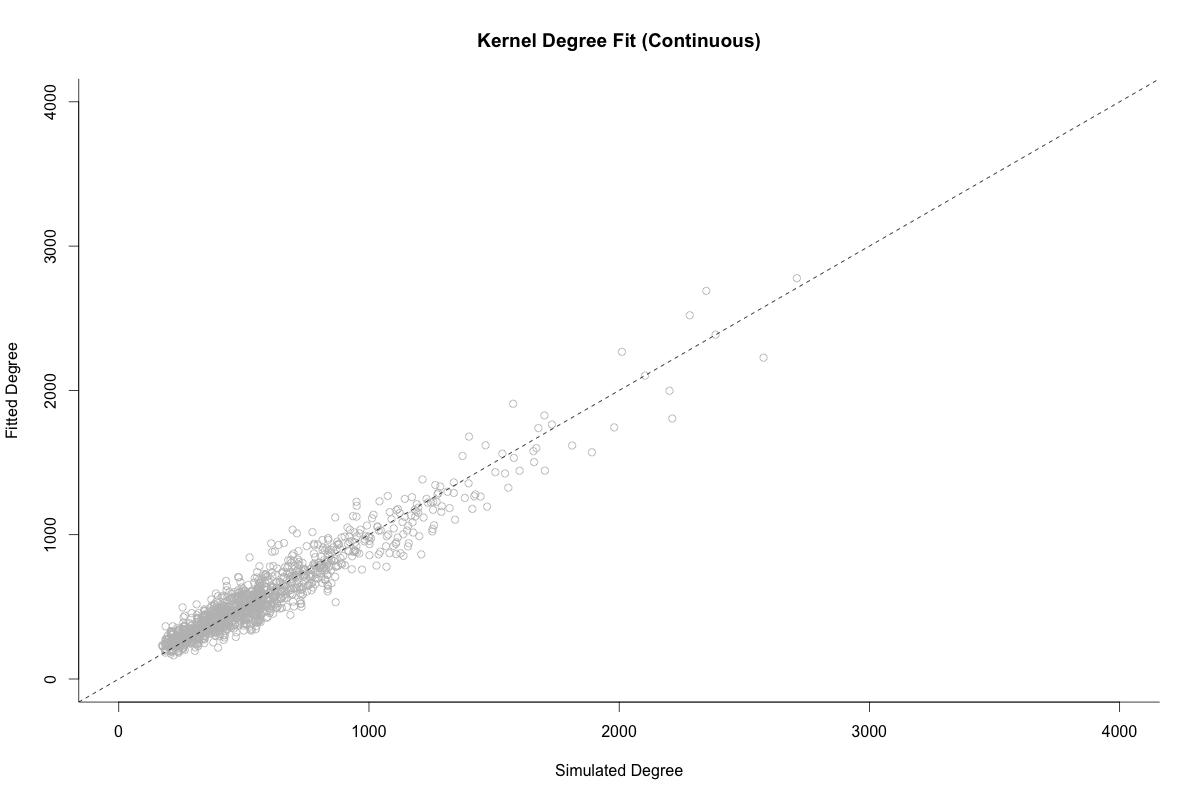
\includegraphics[scale = 0.36]{Estimates_Degree_Continuous.png}

\noindent The degrees are largely underestimated for the discrete model data with a strangely linear offset.

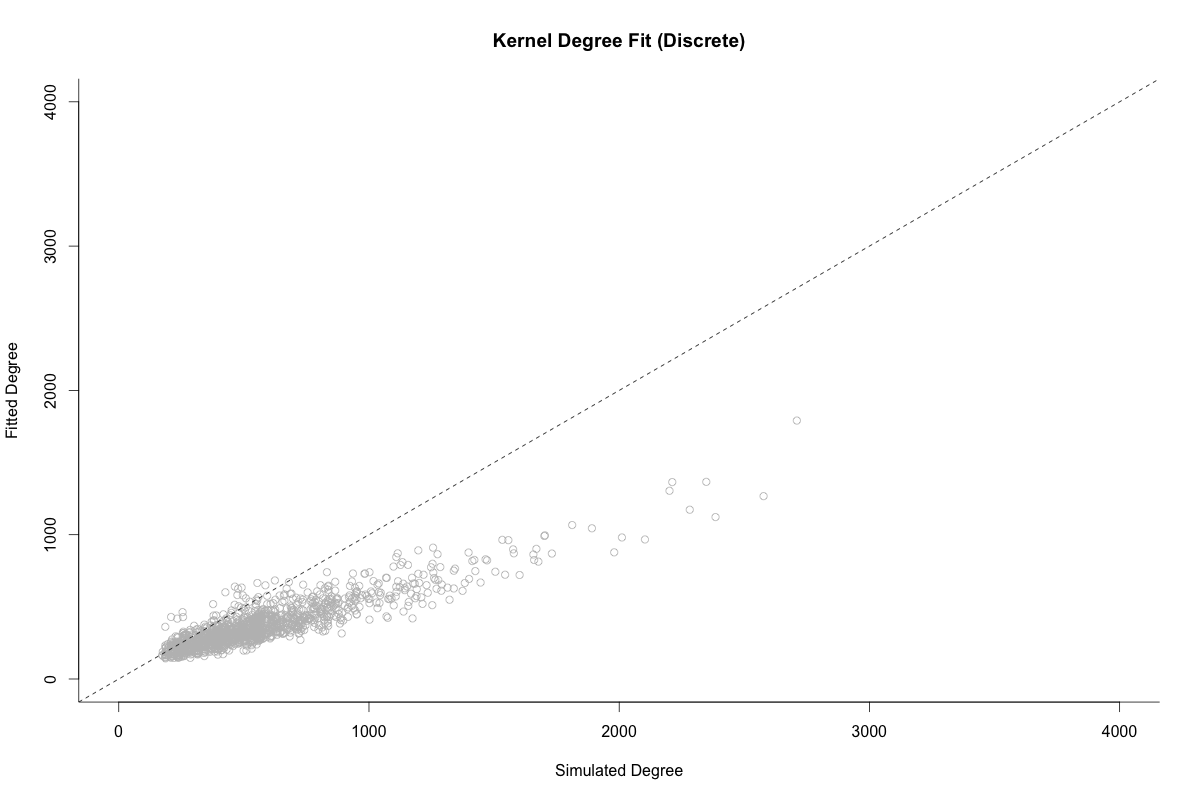
\includegraphics[scale = 0.36]{Estimates_Degree_Discrete.png}

% LAMBDA
\pagebreak
\subsubsection*{Kernel Lengthscale ($\lambda_{g_ig_j}$)}
The continuous model does a great job of recovering the lambdas from the continuous model data.

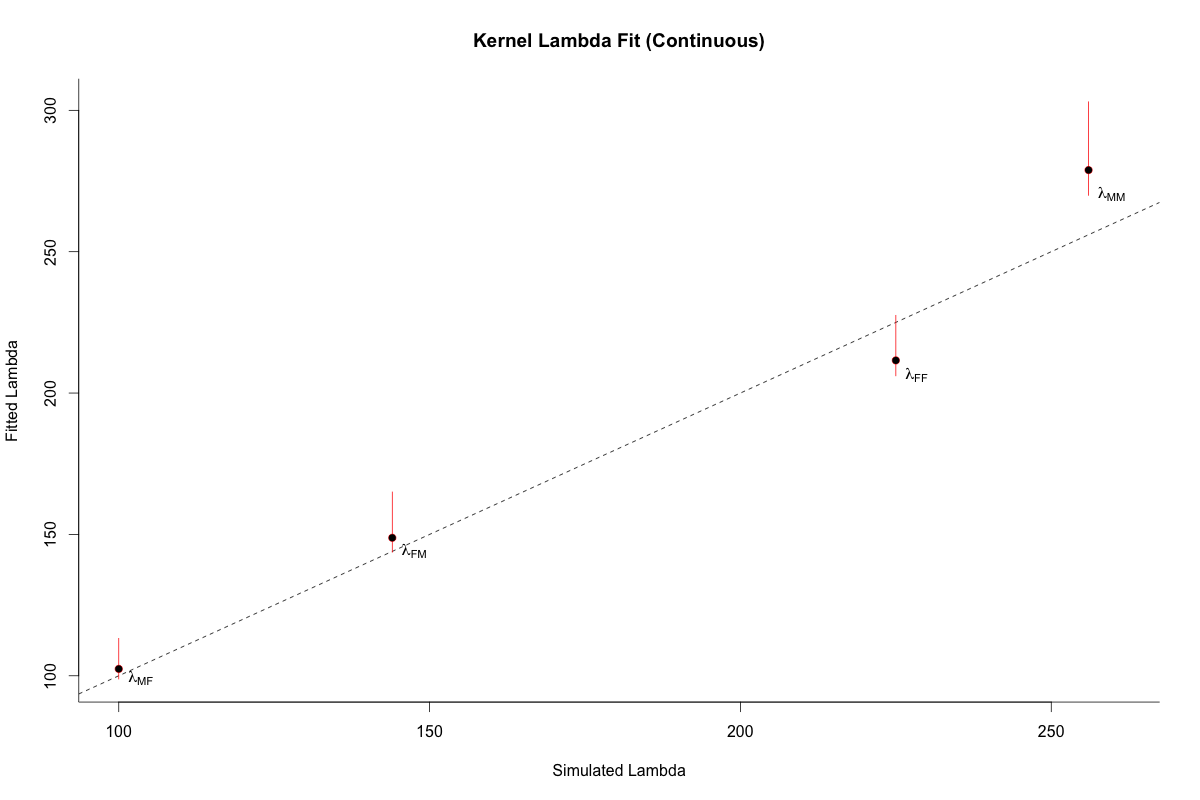
\includegraphics[scale = 0.37]{Estimates_Lambda_Continuous.png}

\noindent The continuous model underestimates the lambdas from the discrete model data.

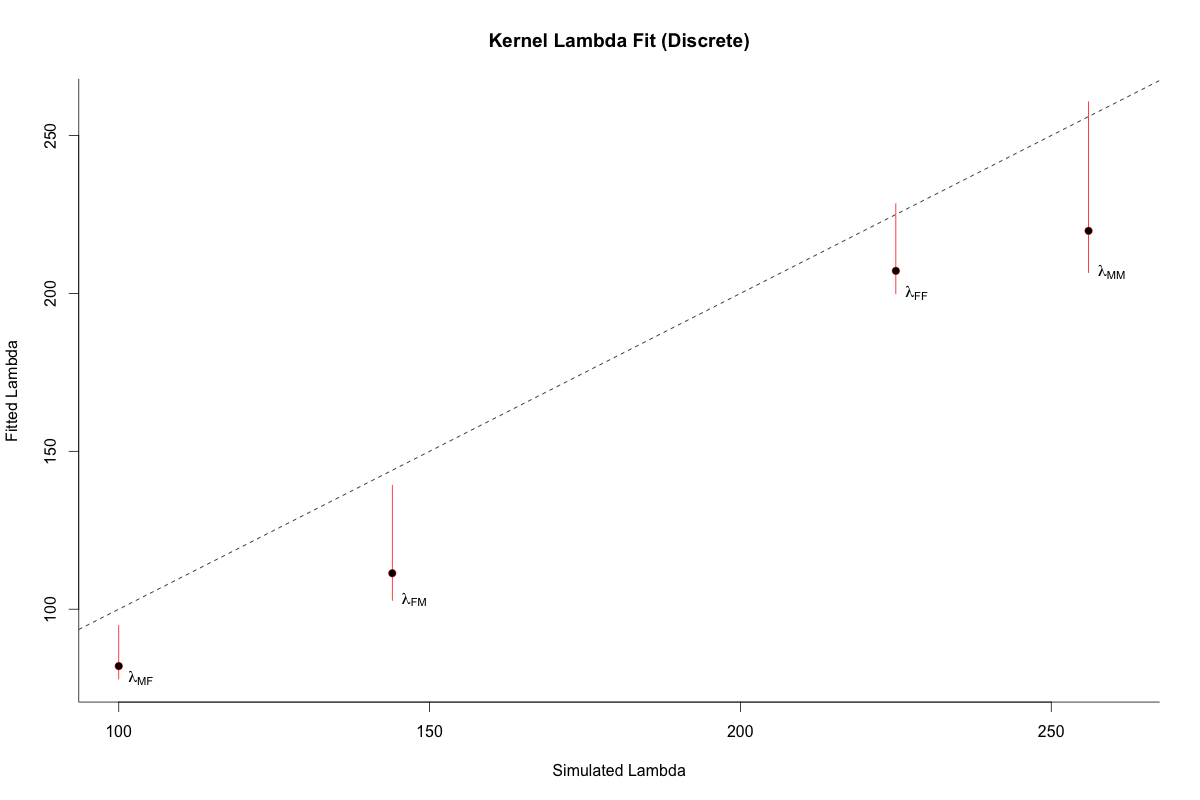
\includegraphics[scale = 0.37]{Estimates_Lambda_Discrete.png}

%OMEGA
\pagebreak
\subsubsection*{Name Overdispersions ($\omega_k$)}
\noindent The overdispersions are also mostly contained within the central 95\% of their posterior distributions, but posterior uncertainty is quite large. Here the posterior median is preferred to the posterior mean.

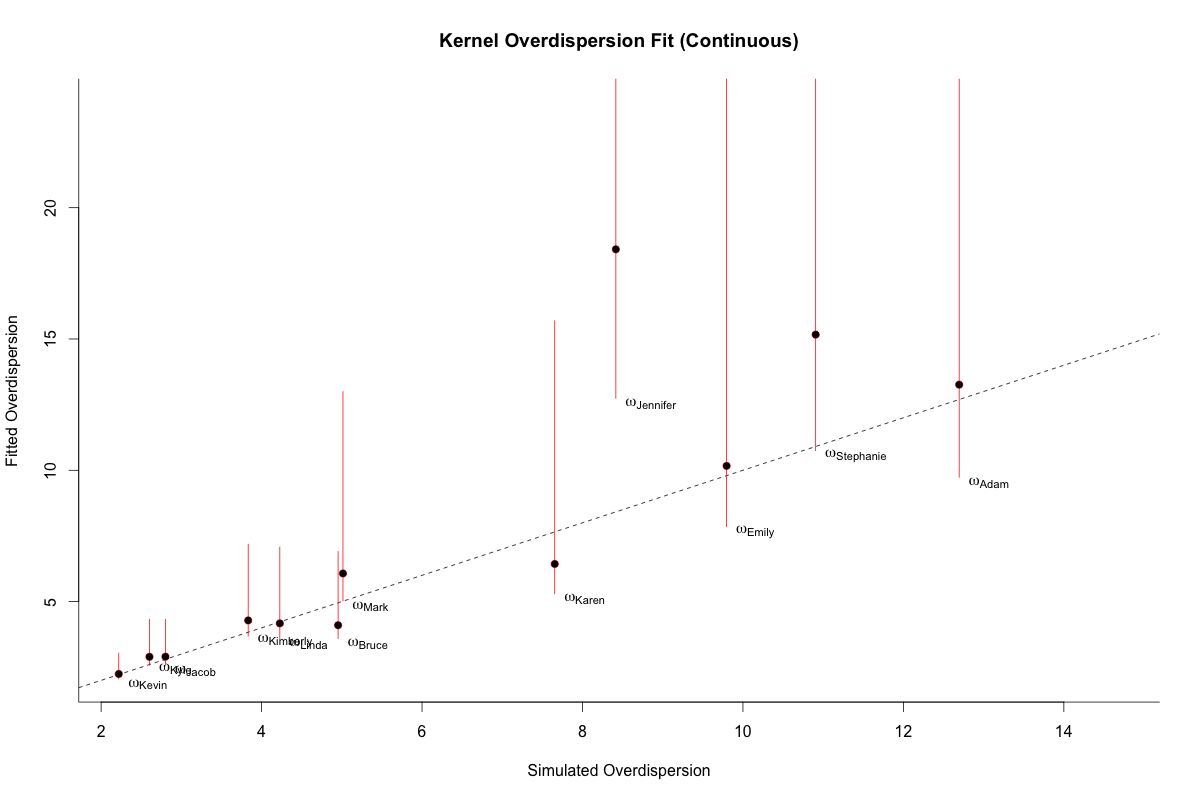
\includegraphics[scale = 0.38]{Estimates_Omega_Continuous.png}

\noindent The overdispersions are poorly recovered from the discrete model data.

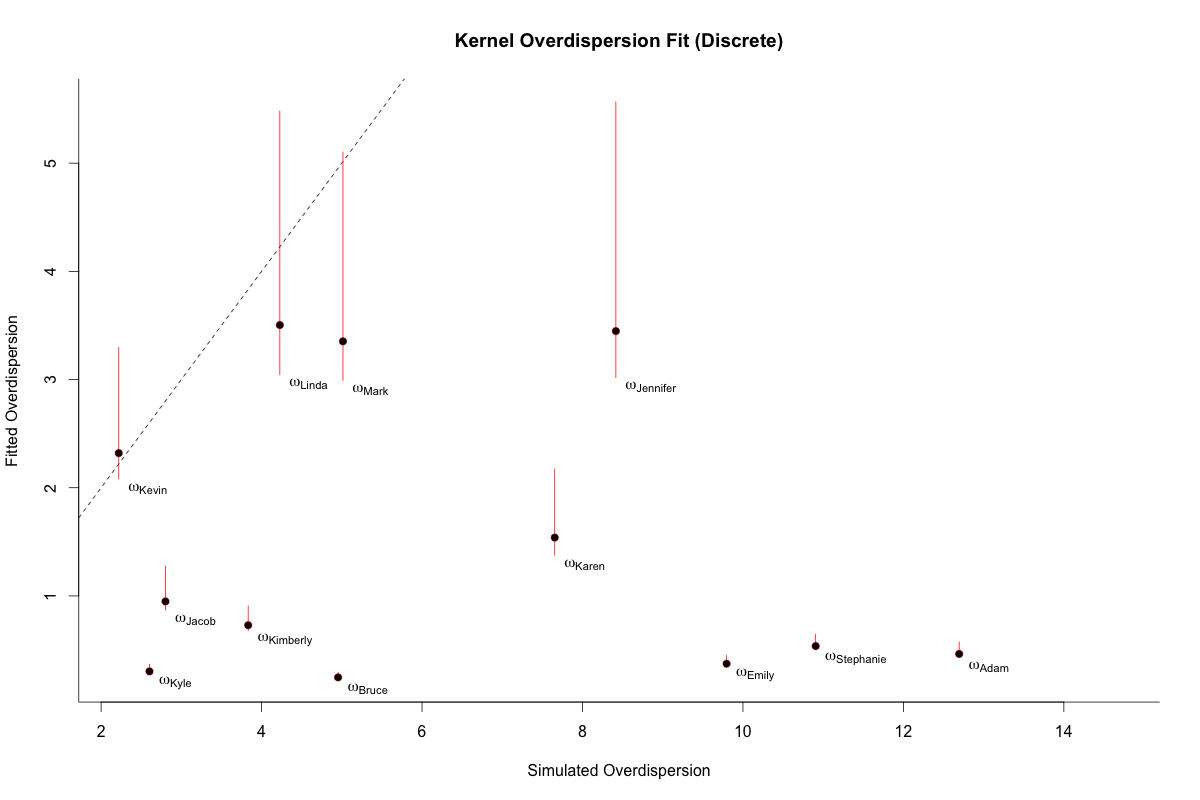
\includegraphics[scale = 0.38]{Estimates_Omega_Discrete.png}

%MIXING%
\pagebreak
\subsubsection*{Gender Mixing Rates ($\rho_{g_ig_k}$)}
\noindent Lastly, the gender mixing rates are recovered very well from the continuous model data.

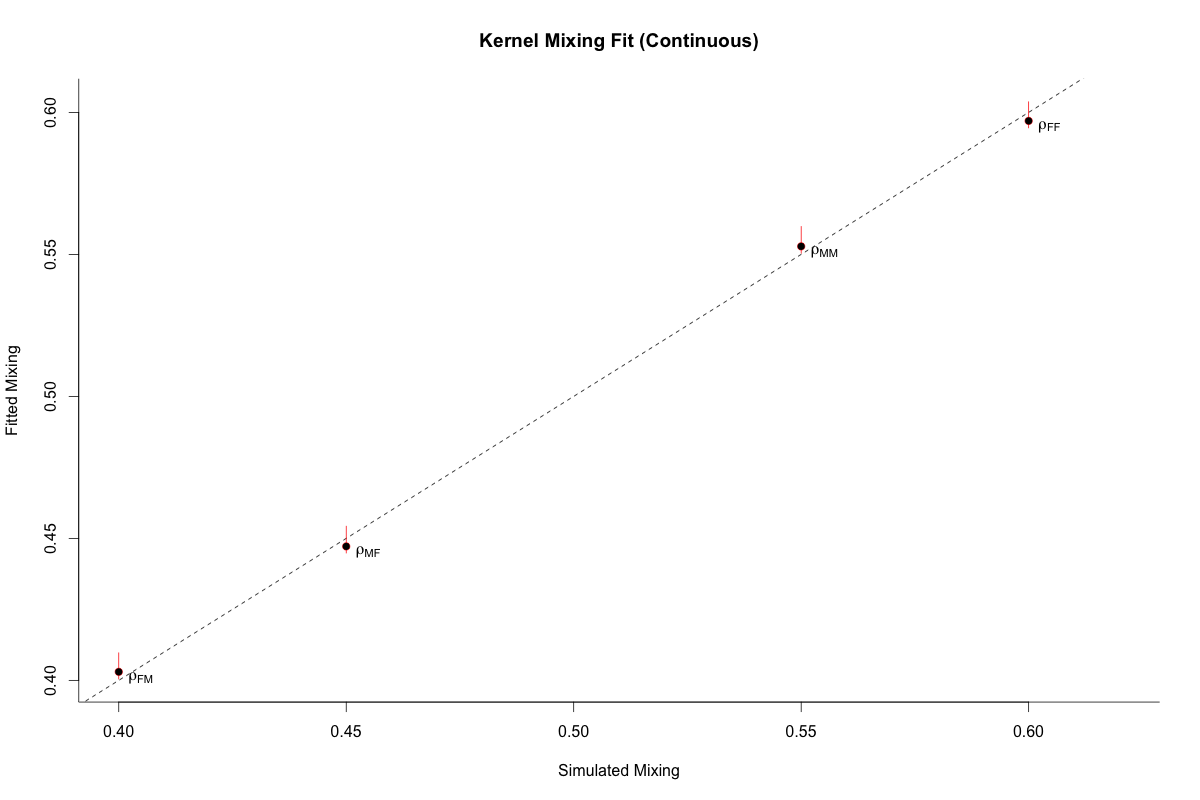
\includegraphics[scale = 0.38]{Estimates_Mixing_Continuous.png}

\noindent However, the mixing is poorly recovered from the discrete model data.

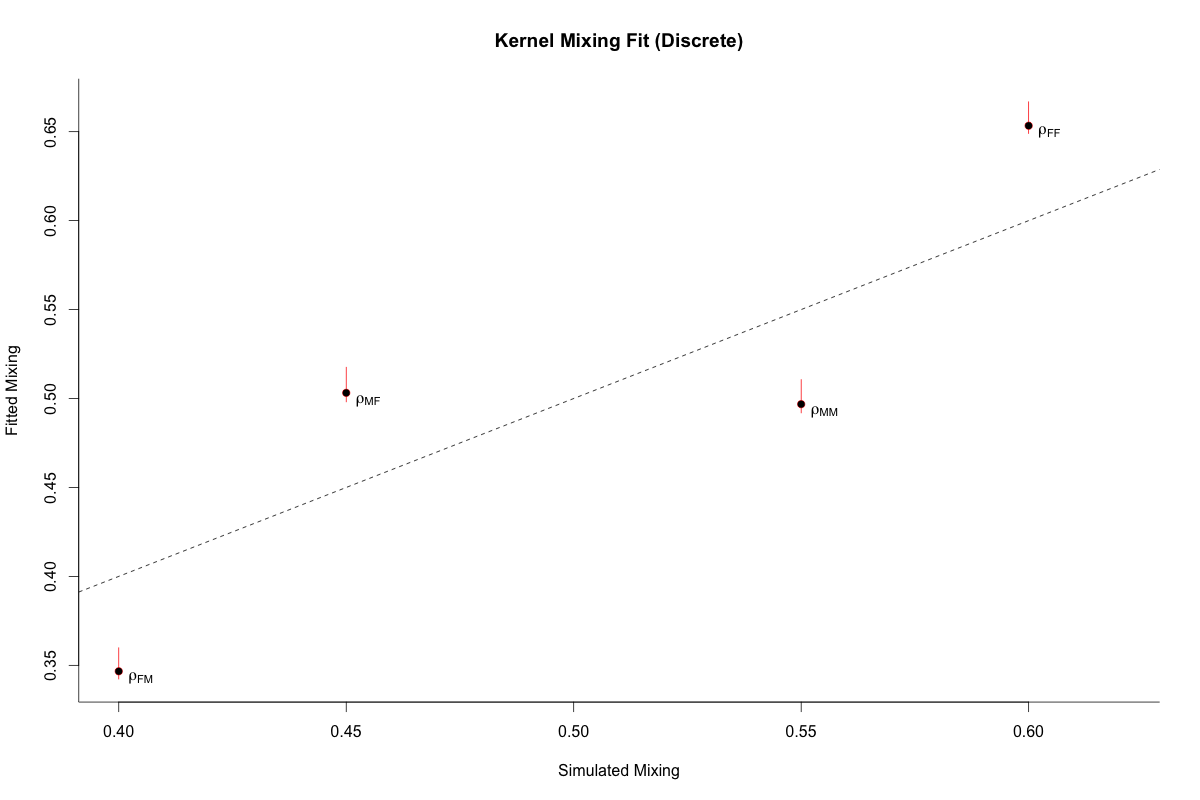
\includegraphics[scale = 0.38]{Estimates_Mixing_Discrete.png}

% OMNI DATA %
\pagebreak
\section{Omni Data Results}
\subsubsection*{Respondent Degrees}
The continuous model estimates imply decreasing network size by age for men, but possibly increasing by age for women.

\begin{center}
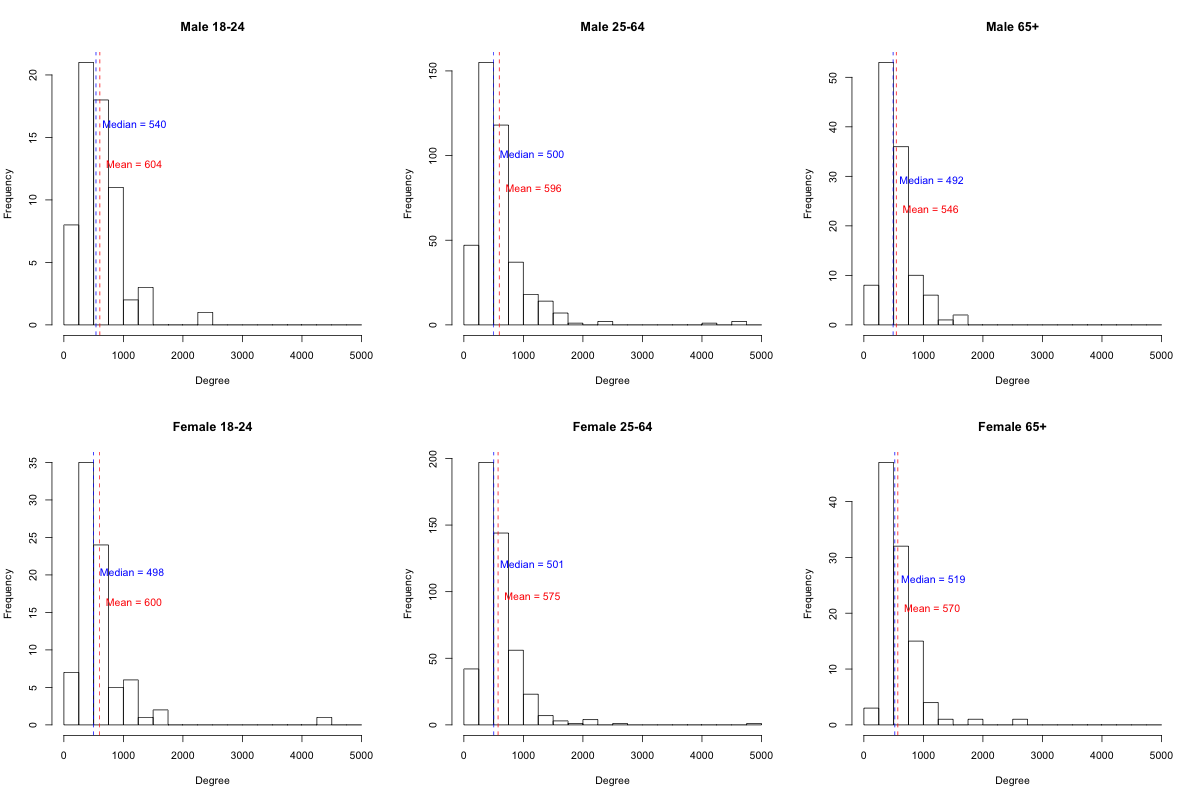
\includegraphics[scale = 0.33]{Estimates_Degree_Omni.png}
\end{center}

\subsubsection*{Kernel Lengthscales}
\noindent The length scales estimated from the actual data are quite large (compared to the ones we choose for the simulated data), implying very flat kernels. The important distinction here, then, is perhaps the relative size of the lengthscales.

$$ \lambda_{BAYES}
= \left( \begin{array}{cc} \lambda_{FF} & \lambda_{FM} \\
\lambda_{MF} & \lambda_{MM} \end{array} \right) 
= \left( \begin{array}{cc}
5092 & 8334 \\
4545 & 13710 \end{array} \right) $$ \vspace{7 pt}

\noindent Indeed, it seems that the female to female kernel is much tighter than the male to male kernel, implying that women tend to know a narrow age range of other women but men tend to know a wide age range of other men. Alternatively, the female to male kernel is much wider than the male to female kernel, implying that women know a wider age range of men while men known a very narrow age range of women.

\subsubsection*{Gender Mixing Rates}
\noindent The gender mixing rates seem to correlate with the kernel lengthscales. Here we see that about 54\% of a female's network is female, while 61\% of a male's network is male. This also implies that females mix more with males than the other way around.

$$ \rho_{BAYES}
= \left( \begin{array}{cc} \rho_{FF} & \rho_{FM} \\
\rho_{MF} & \rho_{MM} \end{array} \right) 
= \left( \begin{array}{cc}
0.54 & 0.46 \\
0.39 & 0.61 \end{array} \right) $$

% MCCARTY DATA %
\pagebreak
\section{McCarty Data Results}
\subsubsection*{Respondent Degrees}
The McCarty data imply network size is a minimum for middle aged men, while it is a maximum for middle aged women.

\begin{center}
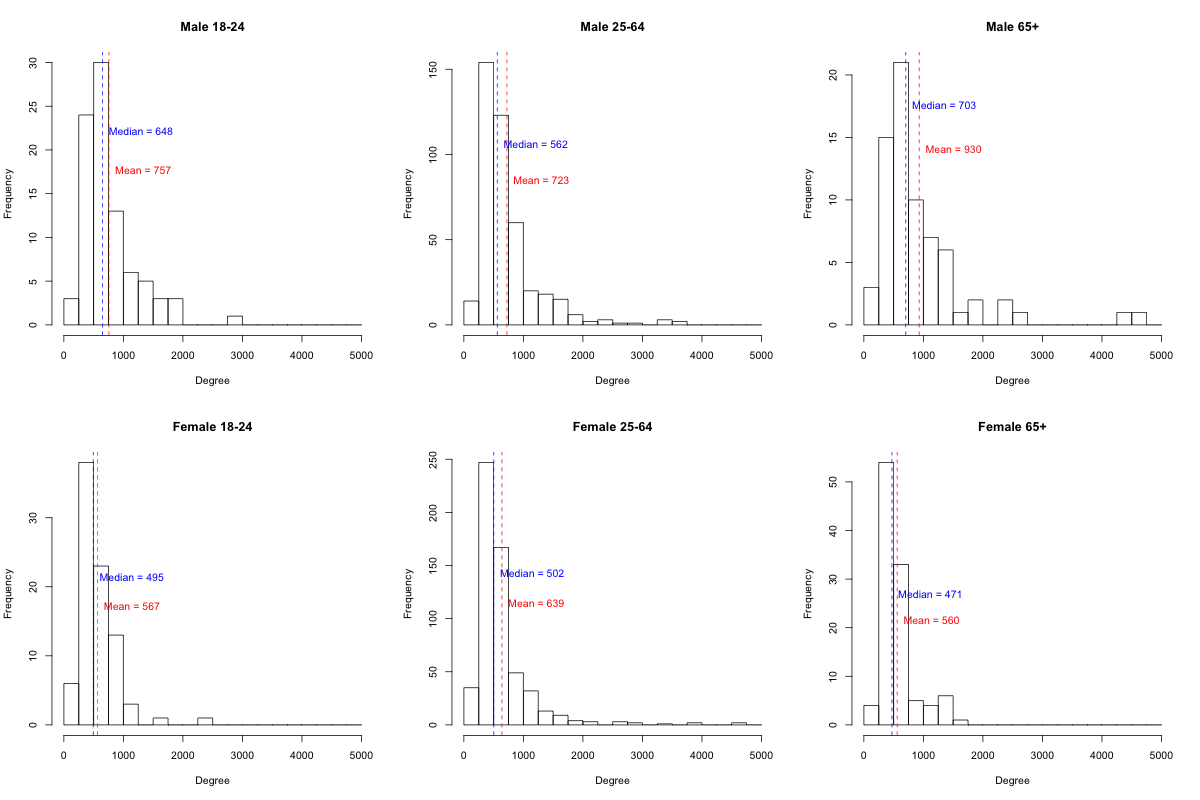
\includegraphics[scale = 0.33]{Estimates_Degree_McCarty.png}
\end{center}

\subsubsection*{Kernel Lengthscales}
\noindent The relative lengthscales for the McCarty data are somewhat similar to the relative lengthscales estimated from the Omni data.

$$ \lambda_{BAYES}
= \left( \begin{array}{cc} \lambda_{FF} & \lambda_{FM} \\
\lambda_{MF} & \lambda_{MM} \end{array} \right) 
= \left( \begin{array}{cc}
1150 & 767 \\
1827 & 1740 \end{array} \right) $$ \vspace{7 pt}

\noindent Namely, we see once again that the female to female kernel is much tighter than the male to male kernel. Additionally, we see once again that the female to male kernel is wider than the male to female kernel.

\subsubsection*{Gender Mixing Rates}
\noindent The gender mixing rates, however, are quite surprising, and don't correlate well with the kernel lengthscales.

$$ \rho_{BAYES}
= \left( \begin{array}{cc} \rho_{FF} & \rho_{FM} \\
\rho_{MF} & \rho_{MM} \end{array} \right) 
= \left( \begin{array}{cc}
0.27 & 0.73 \\
0.31 & 0.69 \end{array} \right) $$

% MCCARTY DATA NO-RECALL %
\pagebreak
\section{McCarty Data Results (Without Michael, Robert, David)}
\subsubsection*{Respondent Degrees}
The McCarty data imply network size is a minimum for middle aged men, while it is a maximum for middle aged women.

\begin{center}
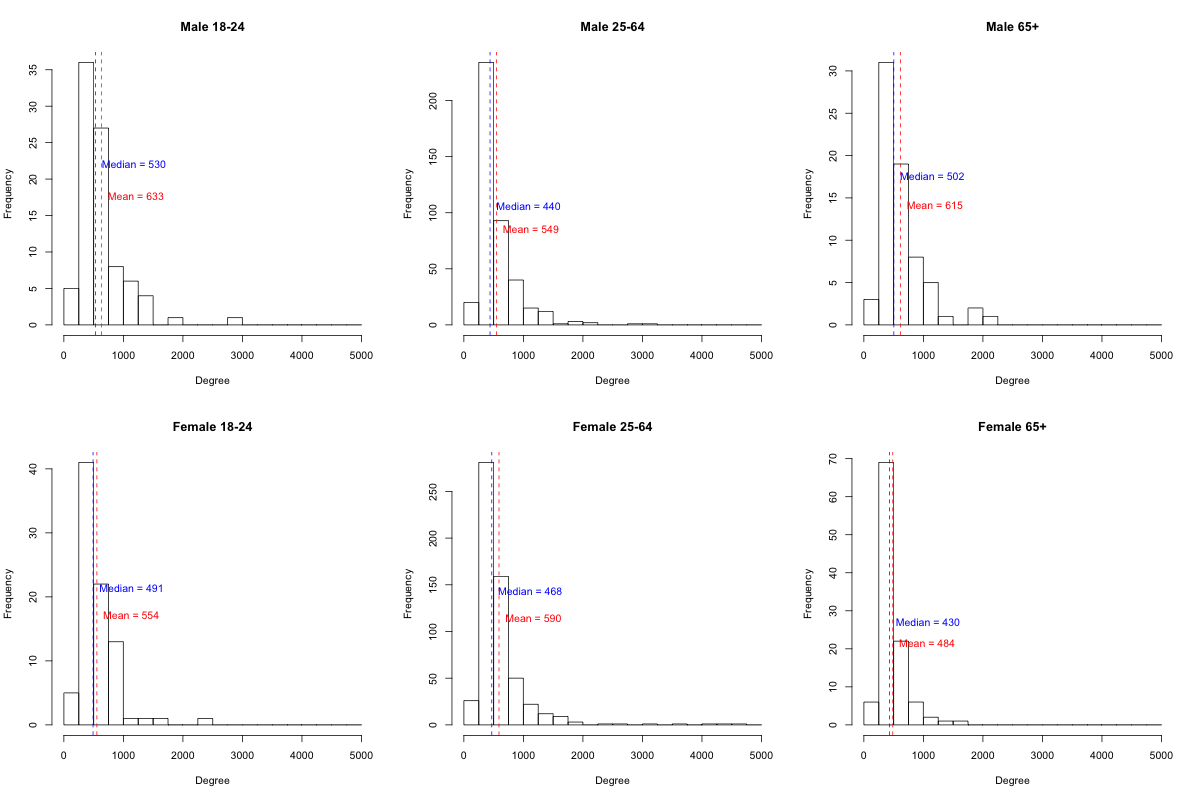
\includegraphics[scale = 0.33]{Estimates_Degree_McCarty_NoRecall.png}
\end{center}

\subsubsection*{Kernel Lengthscales}
\noindent The relative lengthscales for the McCarty data are somewhat similar to the relative lengthscales estimated from the Omni data.

$$ \lambda_{BAYES}
= \left( \begin{array}{cc} \lambda_{FF} & \lambda_{FM} \\
\lambda_{MF} & \lambda_{MM} \end{array} \right) 
= \left( \begin{array}{cc}
2514 & 1483 \\
5064 & 1956 \end{array} \right) $$ \vspace{7 pt}

\noindent Namely, we see once again that the female to female kernel is much tighter than the male to male kernel. Additionally, we see once again that the female to male kernel is wider than the male to female kernel.

\subsubsection*{Gender Mixing Rates}
\noindent The gender mixing rates, however, are quite surprising, and don't correlate well with the kernel lengthscales.

$$ \rho_{BAYES}
= \left( \begin{array}{cc} \rho_{FF} & \rho_{FM} \\
\rho_{MF} & \rho_{MM} \end{array} \right) 
= \left( \begin{array}{cc}
0.30 & 0.70 \\
0.31 & 0.69 \end{array} \right) $$


\end{document}